\documentclass{article}


\usepackage[russian]{babel}
\usepackage{mathtext, amsmath, caption, geometry, amssymb, graphicx, wrapfig}

\usepackage{multirow}
\usepackage{booktabs}
\usepackage{array}
\usepackage{float}
\usepackage{enumitem}
\usepackage{indentfirst}
\usepackage{caption}
\usepackage{pgfplots}

\captionsetup[table]{position=t,justification=raggedleft,slc=off}
%\setlength{\abovecaptionskip}{0pt}
\geometry{margin=1.5cm}

\pgfplotsset{
	every axis/.append style={
		grid=major,
		grid style={line width=.1pt, draw=gray!25},
		tick label style={font=\small},
		label style={font=\small},
		legend style={
			font=\footnotesize,
			fill=white, fill opacity=0.9, text opacity=1,
			draw=gray!40,
			cells={anchor=west}
		}
	}
}

\newcommand{\w}{\vec}

\title{Лабораторная работа №3.3.4. \\ \textbf{Эффект Холла в полупроводниках}}
\author{Данила Шеломанов, Павел Рудачихин, Б04-507}
\date{22.09.2026}

\begin {document}

\maketitle{}

\section {Аннотация} 

	\hspace{4mm} Целью настоящей работы является измерение подвижности и концентрации носителей заряда в образце полупроводника. Исследуется эффект Холла в образце легированного германия: измеряется ЭДС Холла при различных значениях магнитной индукции и тока через образец. По угловому коэффициенту зависимости определяется постоянная Холла, знак которой позволяет установить тип проводимости. Дополнительно измеряется удельная проводимость образца, что даёт возможность вычислить подвижность носителей.
	

\section {Теоретическое введение}

	\subsection{Плотность тока, подвижность носителей и закон Ома}
	
		\hspace{4mm} \textit{Плотность тока} характеризует направленное движение зарядов $q$ в пространстве:
		
		\begin{equation}
			\textbf{j} := qn\textbf{u},
		\end{equation}
		
		где $n$ -- концентрация носителей, $u$ -- скорость дрейфа.
		
		Средняя скорость дрейфа устанавливается постоянной из-за равновесия силы со стороны электрического поля и силы трения о решётку. Введём \textit{подвижность} $\mu$ носителей тока в поле $E$:
		
		\begin{equation}
			\textbf{u} := \mu \textbf{E},
		\end{equation}
		
		В такой модели легко прослеживается связь плотности тока и напряжённости -- \textit{закон Ома}:
		
		\begin{equation}
			\textbf{j} =\sigma\textbf{E}, 
		\end{equation}
		
		где $\sigma = qn\mu$ -- \textit{проводимость} среды.
		

	\subsection{ЭДС Холла однокомпонентной системы}
	
	\begin{figure}[h!]
		\centering
		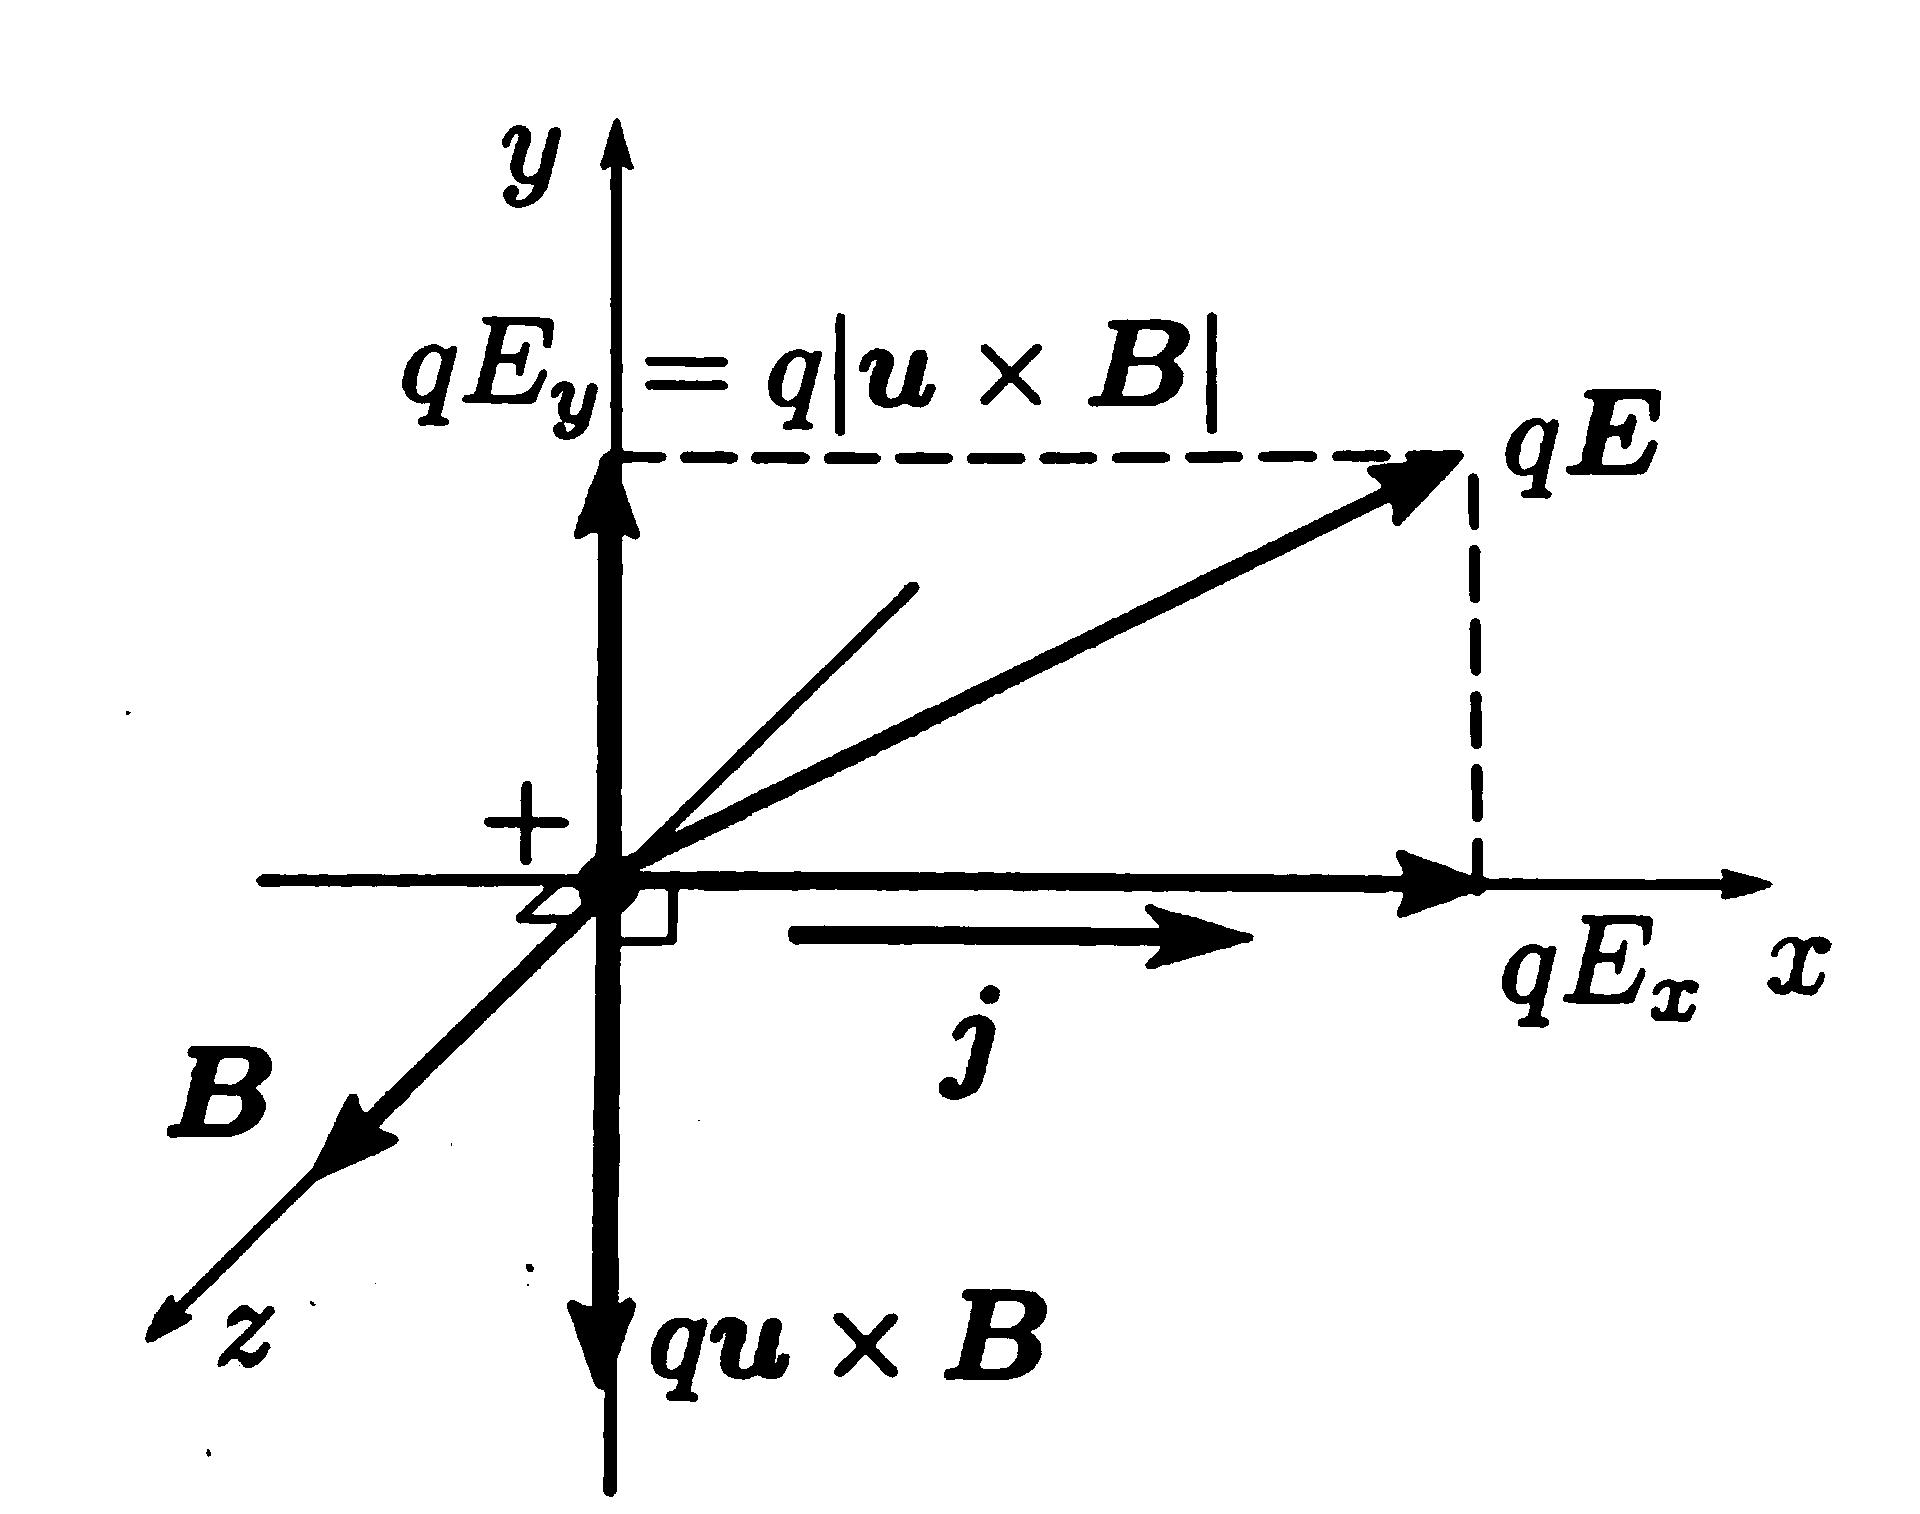
\includegraphics[width=0.3\linewidth]{pic1}
		\caption{Силы, действующие на положительный носитель заряда в проводнике в магнитном поле}
		\label{fig:pic1}
	\end{figure}
	
	\hspace{4mm} Рассмотрим движение положительного носителя заряда в проводнике при наличии магнитного поля (рис. 1).
	
	Силу Лоренца 
	
	\begin{equation}
		\textbf{F}_\Lambda = q (\textbf{v} \times \textbf{B}) .
	\end{equation}
	
	компенсирует сила со стороны электрического поля, созданного отклонившимися к граням проводника носителями заряда (холловского). С учётом этой напряжённости закон Ома можно записать, введя тензор проводимости:
	
	\begin{equation}
		\textbf{{j}} = \hat{\sigma} \textbf{{E}}
	\end{equation}
	
	Тогда холловская напряжённость
	
	\begin{equation}
		E_y = u_x B_z = \frac{j_x}{nq} B_z
	\end{equation}
	
	По оси абсцисс носители будут двигаться, как если бы магнитного поля не было:
	
	\begin{equation}
		j_x = \sigma_0 E_x
	\end{equation}
	
	Полная сила Лоренца уравновешена трением среды:
	
	\begin{equation}
		q(\textbf{E} + \textbf{v} \times \textbf{B}) = \frac{q\textbf{u}}{\mu}
	\end{equation}
	
	С учётом введённых выше обозначений получаем \textit{обобщённый закон Ома}
	
	\begin{equation}
		\textbf{E} = \frac{\textbf{j}}{\sigma_0} - \frac{1}{nq} \textbf{j} \times \textbf{B}
	\end{equation}
	
	Вводя тензор удельного сопротивления $\hat{\rho}$, получаем
	
	\begin{equation}
		\textbf{E} = \hat{\rho}\textbf{j} = \begin{pmatrix}
			1 & -\mu B & 0 \\
			\mu B & 1 & 0 \\
			0 & 0 & 1 \\
		\end{pmatrix} \frac{\textbf{j}}{\sigma_0}
	\end{equation}
	
	Обратив матрицу, имеем
	
	\begin{equation}
		\hat{\sigma} = \frac{\sigma_0}{1 + (\mu B)^2} \begin{pmatrix}
			1 & \mu B & 0 \\
			-\mu B & 1 & 0 \\
			0 & 0 & 1 \\
		\end{pmatrix}
	\end{equation}
	
	
	
	\subsection{Мостик Холла}
	
	\begin{figure}[h!]
		\centering
		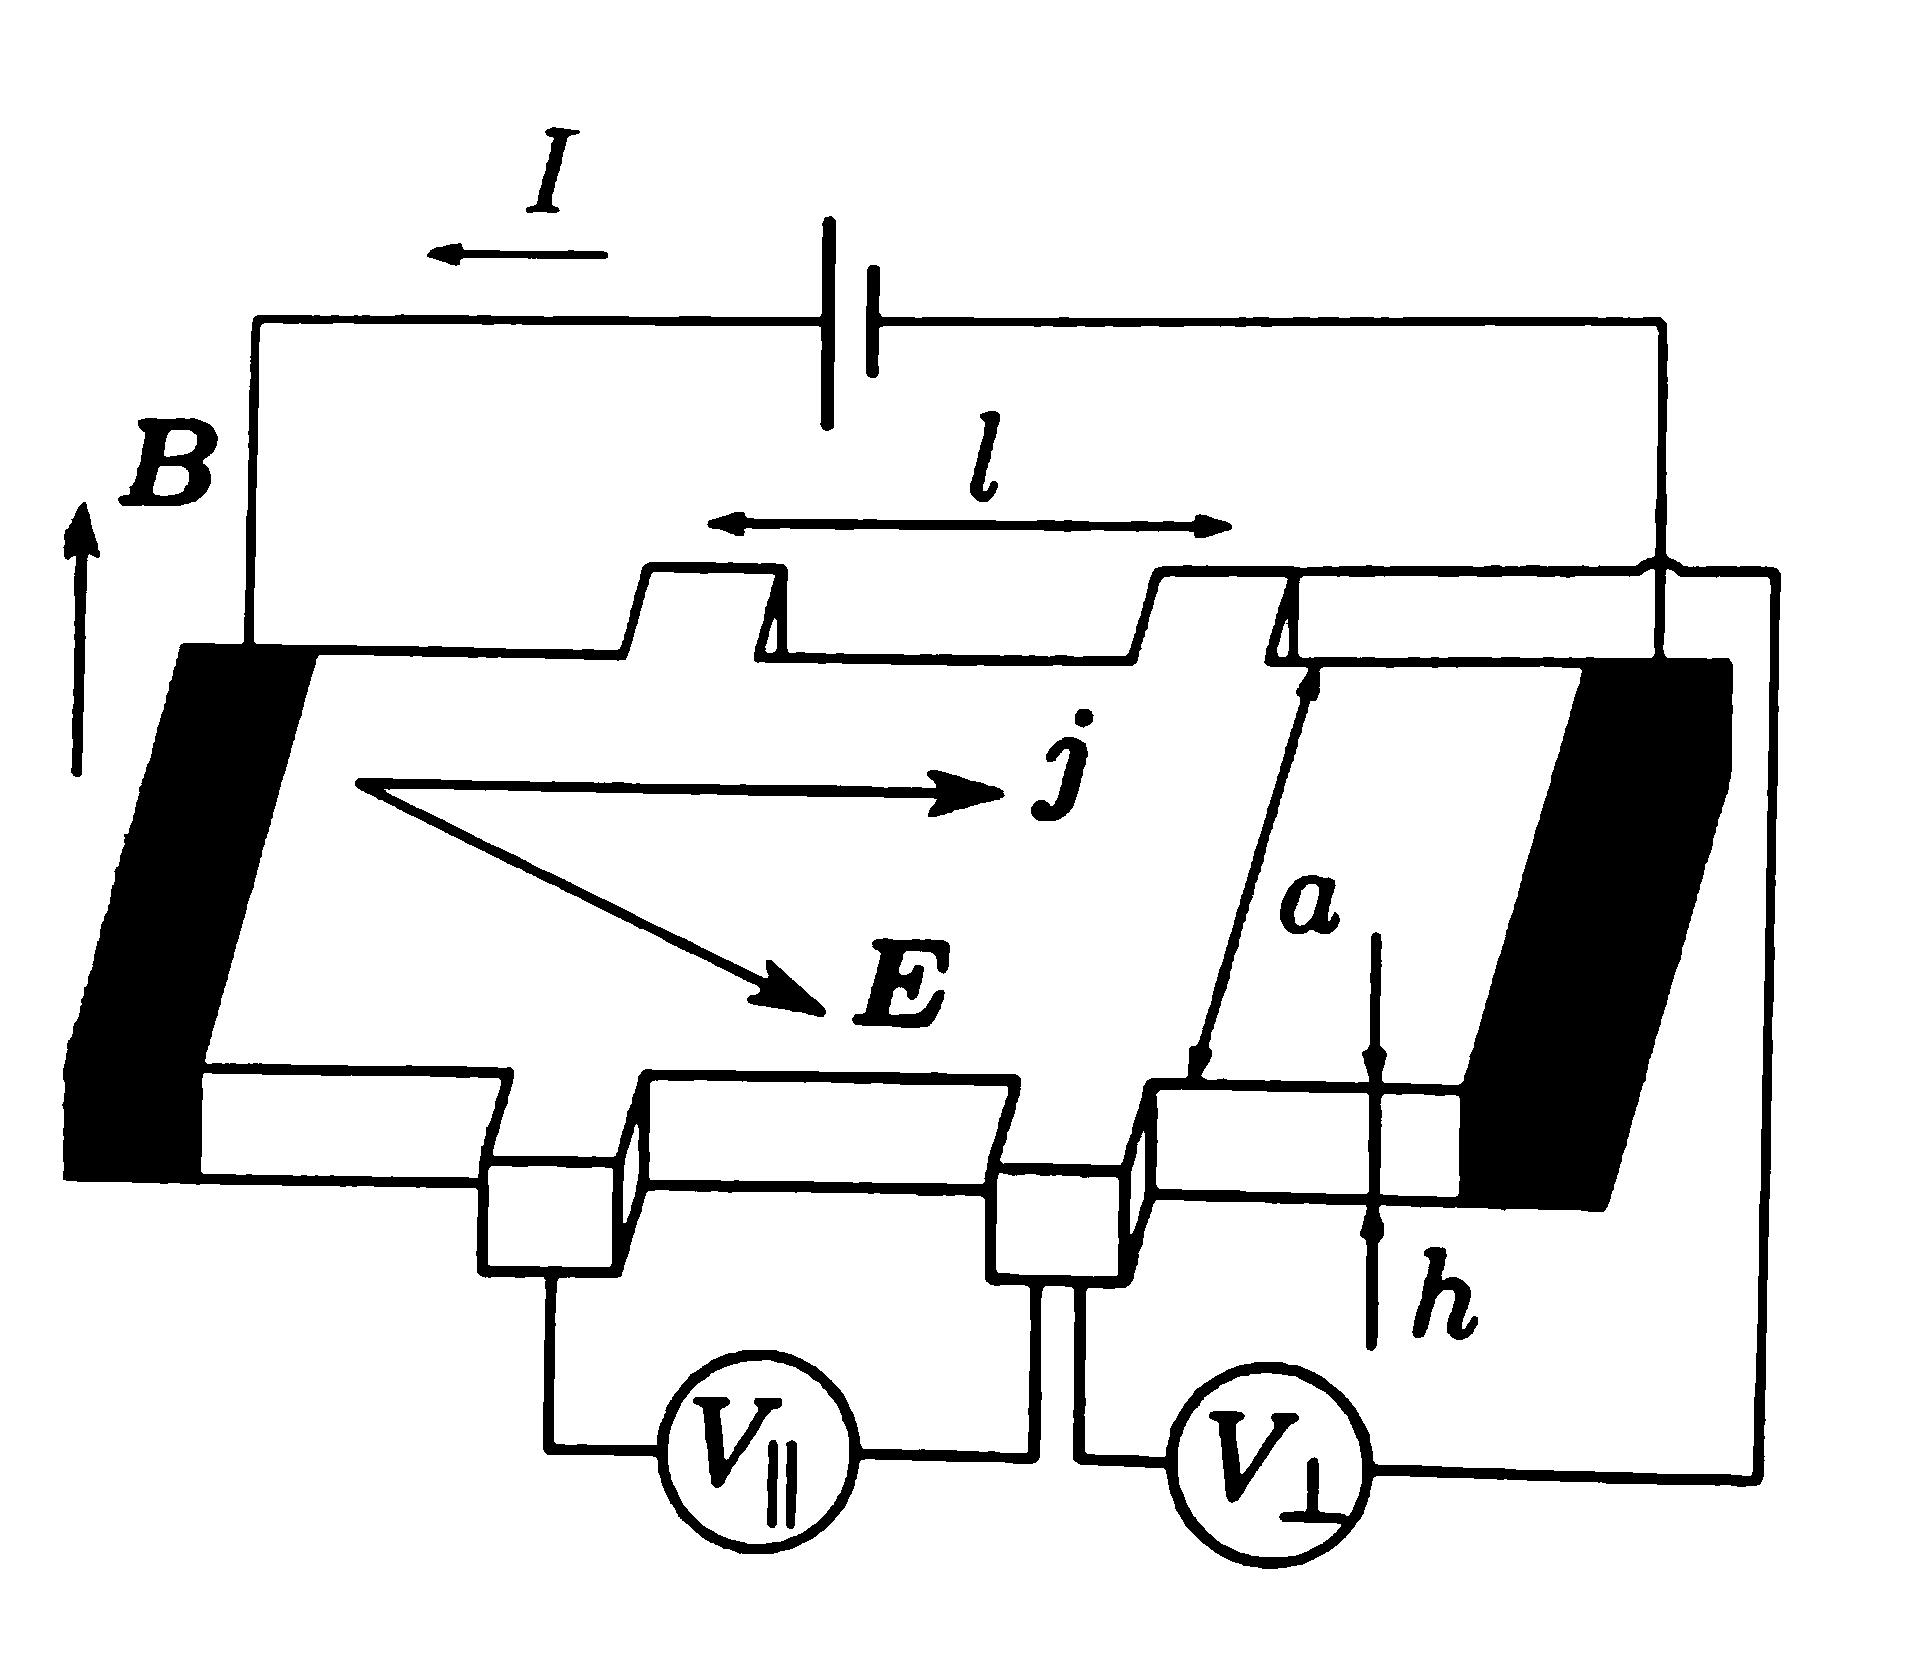
\includegraphics[width=0.5\linewidth]{pic2}
		\caption{Мостик Холла}
		\label{fig:pic2}
	\end{figure}
	
	В настоящей работе геометрия исследуемого образца соответствует мостику Холла (см. рис. 2). Холловское напряжение:
	
	\begin{equation}
		U_{\perp} = E_ya = \frac{j_xBa}{nq} = \frac{B}{nqh}I = R_H \frac{B}{h}I
	\end{equation}
	
	где $R_H$ -- константа Холла.
	
	Напряжение вдоль пластинки:
	
	\begin{equation}
		U_{||} = E_xl = \frac{j_xl}{\sigma_0} = IR_0
	\end{equation}
	
	где $R_0$ -- омическое сопротивление образца.
	
	
	
	
\section{Описание установки}

	\begin{figure}[h!]
		\centering
		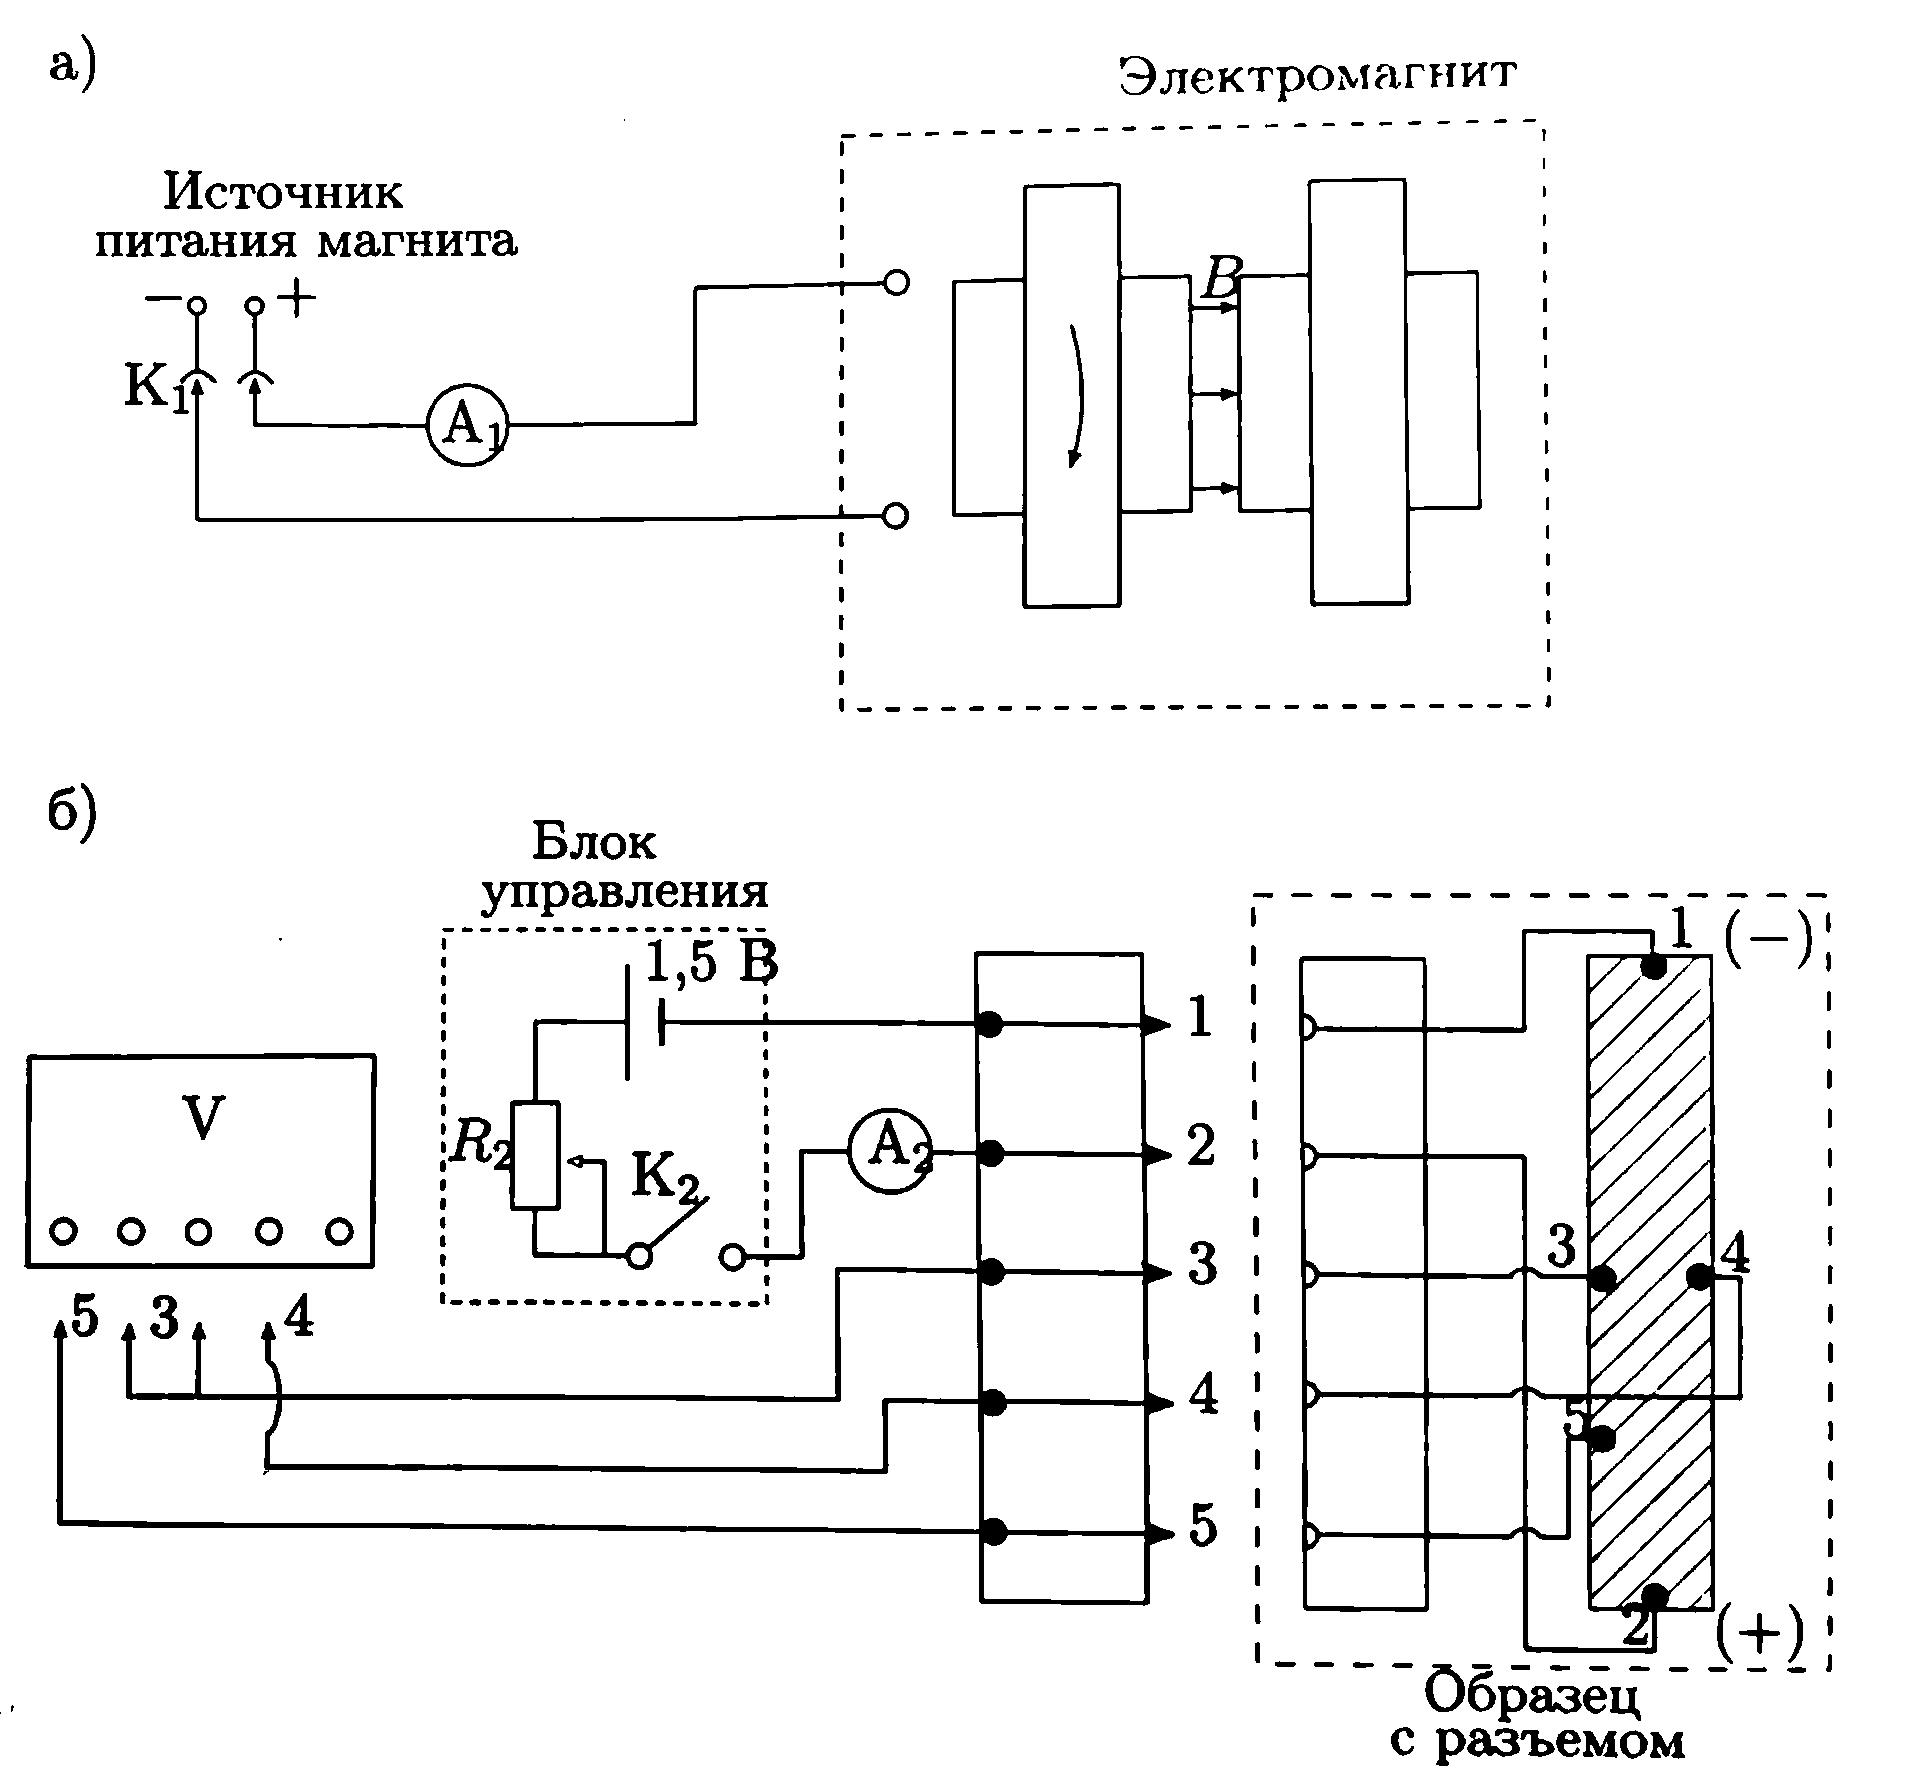
\includegraphics[width=0.7\linewidth]{setup}
		\caption{Схема установки}
		\label{fig:setup}
	\end{figure}
	
	Схема установки включает источник питания электромагнита, блок управления и образец германия с разъёмами. Для измерений используются миллиамперметр, милливеберметр, цифровой вольтметр В7-78/1.
	
	Параметры исследуемого образца: $a = 2$ мм, $l = 8$ мм и $L_{35} = 15$ мм.
	
\section{Результаты и обсуждения}

\subsection{Калибровка электромагнита}
Для определения связи между индукцией магнитного поля $B$ в зазоре электромагнита и током $I_M$ через обмотку проведена калибровка. Магнитный поток измеряется милливеберметром: $\Phi = B S N$. Результаты приведены в таблице~\ref{tab:calib} и на рисунке~\ref{fig:calib}. Погрешность милливеберметра рассчитана по формуле

\begin{equation}
	\delta\Phi = 0,005\Phi + 2 \text{мВб}
\end{equation}

Погрешность для амперметра на источнике положена $\delta I_M = 0,03$ А



\begin{figure}[H]
	\centering
	\begin{tikzpicture}
		\begin{axis}[
			width=0.85\textwidth, height=6.5cm,
			xlabel={$I_M$, А}, ylabel={$B$, Тл},
			legend pos=north west,
			xmin=0, xmax=2.2, ymin=0
			]
			\addplot[color=blue, mark=*, thick] coordinates {
				(0.13, 0.100) (0.26, 0.157) (0.39, 0.257) (0.52, 0.343)
				(0.65, 0.414) (0.78, 0.500) (0.91, 0.571) (1.04, 0.643)
				(1.17, 0.714) (1.30, 0.771) (1.43, 0.814) (1.56, 0.857)
				(1.69, 0.900) (1.82, 0.929) (1.95, 0.957) (2.08, 0.986) (2.10, 0.986)
			};
			\legend{Калибровка $B(I_M)$}
		\end{axis}
	\end{tikzpicture}
	\caption{График калибровки электромагнита}
	\label{fig:calib}
\end{figure}


\subsection{Измерение ЭДС Холла}
Снята зависимость напряжения $|U_{34}|$ от магнитной индукции $B$. При $I_M = 0$ напряжение не равно нулю: $U_{034} = 0{,}360$ мВ, поэтому далее рассматривается $|U_{34}|$ с учётом этой поправки. Серия экспериментов проведена для различных токов через образец $I$ (от $0{,}2$ до $1{,}1$ мА). Все измеренные значения напряжений имели отрицательный знак. Результаты приведены в таблице~\ref{tab:hall}, соответствующие зависимости — на рисунке~\ref{fig:hall}.



\begin{figure}[H]
	\centering
	\begin{tikzpicture}
		\begin{axis}[
			width=0.92\textwidth, height=9.5cm,
			xlabel={$B$, Тл}, ylabel={$|U_{34}|$, мВ},
			xmin=0, xmax=1.0, ymin=0,
			legend columns=2,
			legend style={at={(0.02,0.98)}, anchor=north west}
			]
			\addplot[only marks, mark=*, color=blue] coordinates {
				(0.000,0.069) (0.100,0.339) (0.257,0.944) (0.414,1.513) (0.571,2.027) (0.714,2.473) (0.814,2.825) (0.900,3.053) (0.957,3.225)};
			\addplot[domain=0:1, color=blue, thick, no marks] {3.30*x + 0.10};
			\addlegendentry{$I=0.20$ мА}
			
			\addplot[only marks, mark=square*, color=red] coordinates {
				(0.000,0.115) (0.100,0.719) (0.257,1.828) (0.414,2.971) (0.571,3.997) (0.714,4.871) (0.814,5.532) (0.900,5.987) (0.957,6.298)};
			\addplot[domain=0:1, color=red, thick, no marks] {6.48*x + 0.15};
			\addlegendentry{$I=0.40$ мА}
			
			\addplot[only marks, mark=triangle*, color=brown] coordinates {
				(0.000,0.157) (0.100,0.999) (0.257,2.538) (0.414,4.115) (0.571,5.569) (0.714,6.722) (0.814,7.598) (0.900,8.208) (0.957,8.687)};
			\addplot[domain=0:1, color=brown, thick, no marks] {8.94*x + 0.18};
			\addlegendentry{$I=0.55$ мА}
			
			\addplot[only marks, mark=diamond*, color=green!60!black] coordinates {
				(0.000,0.200) (0.100,1.263) (0.257,3.222) (0.414,5.231) (0.571,6.977) (0.714,8.515) (0.814,9.682) (0.900,10.441) (0.957,11.029)};
			\addplot[domain=0:1, color=green!60!black, thick, no marks] {11.35*x + 0.22};
			\addlegendentry{$I=0.70$ мА}
			
			\addplot[only marks, mark=pentagon*, color=orange] coordinates {
				(0.000,0.261) (0.100,1.568) (0.257,4.136) (0.414,6.751) (0.571,9.056) (0.714,10.991) (0.814,12.495) (0.900,13.485) (0.957,14.244)};
			\addplot[domain=0:1, color=orange, thick, no marks] {14.65*x + 0.28};
			\addlegendentry{$I=0.90$ мА}
			
			\addplot[only marks, mark=star, color=magenta] coordinates {
				(0.000,0.325) (0.100,1.822) (0.257,5.152) (0.414,8.143) (0.571,10.972) (0.714,13.342) (0.814,15.182) (0.900,16.419) (0.957,17.317)};
			\addplot[domain=0:1, color=magenta, thick, no marks] {17.85*x + 0.35};
			\addlegendentry{$I=1.10$ мА}
			
			\addplot[only marks, mark=x, color=gray] coordinates {
				(0.000,0.325) (0.100,1.815) (0.257,5.062) (0.414,8.142) (0.571,10.931) (0.714,13.365) (0.814,15.180) (0.900,16.215) (0.957,17.165)};
			\addplot[domain=0:1, color=gray, dashed, thick, no marks] {17.65*x + 0.35};
			\addlegendentry{$I=1.10$ мА (повт.)}
		\end{axis}
	\end{tikzpicture}
	\caption{Семейство зависимостей ЭДС Холла от индукции магнитного поля при различных токах через образец}
	\label{fig:hall}
\end{figure}

Из рисунка~\ref{fig:hall} видно, что при фиксированном токе $I$ напряжение $|U_{34}|$ линейно растёт с индукцией $B$, а наклон прямых увеличивается пропорционально току. Это качественно согласуется с формулой (2).

\subsection{Определение постоянной Холла}
Угловые коэффициенты аппроксимирующих прямых $k = \mathrm{d}U/\mathrm{d}B$ (рис.~\ref{fig:hall}) сведены в таблицу~\ref{tab:k}. График зависимости $k = f(I)$ приведён на рисунке~\ref{fig:k}.

\begin{table}[H]
	\centering
	\caption{Угловые коэффициенты аппроксимирующих прямых}
	\label{tab:k}
	\begin{tabular}{c ccccc}
		\toprule
		$I$, мА   & 0.20 & 0.40 & 0.55 & 0.70 & 0.90 \\
		\midrule
		$k$, мВ/Тл & 3.30 & 6.48 & 8.94 & 11.35 & 14.65 \\
		\bottomrule
	\end{tabular}
	\qquad
	\begin{tabular}{c c}
		\toprule
		$I$, мА & $k$, мВ/Тл \\
		\midrule
		1.10 & 17.85 \\
		1.10\textsuperscript{*} & 17.65 \\
		\bottomrule
	\end{tabular}
	\par\vspace{2pt}
	{\footnotesize\textsuperscript{*} повторное измерение}
\end{table}

\begin{figure}[H]
	\centering
	\begin{tikzpicture}
		\begin{axis}[
			width=0.75\textwidth, height=6cm,
			xlabel={$I$, мА}, ylabel={$k$, мВ/Тл},
			legend pos=north west,
			xmin=0, xmax=1.2, ymin=0
			]
			\addplot[only marks, mark=*, color=blue] coordinates {
				(0.20, 3.30) (0.40, 6.48) (0.55, 8.94) (0.70, 11.35) (0.90, 14.65) (1.10, 17.85)
			};
			\addplot[domain=0:1.2, color=red, thick, no marks] {16.15*x + 0.05};
			\legend{Эксперимент, $k(I) = 16{,}15 \cdot I$}
		\end{axis}
	\end{tikzpicture}
	\caption{Зависимость углового коэффициента от тока}
	\label{fig:k}
\end{figure}

По графику найдём постоянную Холла $R_x$. Угловой коэффициент прямой $K = \mathrm{d}k/\mathrm{d}I = 16{,}15$ В/(Тл$\cdot$А). Погрешность рассчитана по методу наименьших квадратов:
\begin{equation}
	R_x = -K a = -16{,}15 \cdot 2{,}2\cdot 10^{-3}
	= -(3{,}55 \pm 0{,}24)\cdot 10^{-2}\ \text{м}^3/\text{Кл}.
\end{equation}
Относительная погрешность составляет $6{,}8\%$.

\subsection{Определение типа проводимости}
С учётом направления тока в образце и отрицательного знака ЭДС Холла по правилу векторного произведения получаем, что проводимость образца — \textbf{электронная} ($n$-тип).

\subsection{Концентрация, проводимость и подвижность носителей}
Концентрация носителей тока рассчитывается как
\begin{equation}
	n = \frac{1}{|R_x|\,e} = (1{,}76 \pm 0{,}12)\cdot 10^{20}\ \text{м}^{-3}.
\end{equation}

По формуле (3) рассчитаем удельную проводимость образца. При $I = 1{,}1$ мА, $U_{35} = 0{,}345$ В и параметрах установки $a = 2{,}2$ мм, $l = 7$ мм, $L_{34} = 3$ мм:
\begin{equation}
	\sigma = \frac{I\,L_{34}}{U_{35}\,a\,l}
	= 8{,}70\ \text{(Ом}\cdot\text{м)}^{-1}.
\end{equation}

Подвижность носителей в образце:
\begin{equation}
	b = \sigma\,|R_x| = (3088 \pm 260)\ \text{см}^2/(\text{В}\cdot\text{с}).
\end{equation}
Теоретическое значение для электронной проводимости чистого германия: $b_{\text{теор}} = 3800$ см$^2$/(В$\cdot$с).
	
\section{Выводы}

В ходе работы был исследован эффект Холла в полупроводнике германия $n$-типа. Определены следующие характеристики образца:
\begin{itemize}
	\item постоянная Холла $R_x = -3{,}55\cdot 10^{-2}$ м$^3$/Кл;
	\item концентрация электронов $n = 1{,}76\cdot 10^{20}$ м$^{-3}$;
	\item удельная электрическая проводимость $\sigma = 8{,}70$ (Ом$\cdot$м)$^{-1}$;
	\item подвижность носителей $b \approx 3090$ см$^2$/(В$\cdot$с).
\end{itemize}

Результаты совпадают с табличными по порядку величины. Небольшое отличие экспериментального значения подвижности от теоретического объясняется наличием примесей в легированном германии, которые снижают подвижность за счёт дополнительного рассеяния носителей заряда. Среди систематических погрешностей наибольшей в относительном выражении оказалась погрешность милливеберметра. Однако основной вклад в погрешность результатов статистический, определённый по МНК. Возможно, следовало бы получить больше экспериментальных значений, что уменьшило бы статистическую погрешность.

\section{Приложение}

\begin{table}[H]
	\centering
	\caption{Калибровка электромагнита}
	\label{tab:calib}
	\resizebox{\textwidth}{!}{%
		\begin{tabular}{l *{17}{c}}
			\toprule
			$I_M$, А    & 0.13 & 0.26 & 0.39 & 0.52 & 0.65 & 0.78 & 0.91 & 1.04 & 1.17 & 1.30 & 1.43 & 1.56 & 1.69 & 1.82 & 1.95 & 2.08 & 2.10 \\
			$\Phi$, мВб & 7    & 11   & 18   & 24   & 29   & 35   & 40   & 45   & 50   & 54   & 57   & 60   & 63   & 65   & 67   & 69   & 69   \\
			$B$, Тл     & 0.100 & 0.157 & 0.257 & 0.343 & 0.414 & 0.500 & 0.571 & 0.643 & 0.714 & 0.771 & 0.814 & 0.857 & 0.900 & 0.929 & 0.957 & 0.986 & 0.986 \\
			\bottomrule
		\end{tabular}%
	}
\end{table}	
\begin{table}[H]
	\centering
	\caption{Зависимость напряжения $|U_{34}|$ (мВ) от индукции поля $B$ (Тл)}
	\label{tab:hall}
	\small
	\setlength{\tabcolsep}{5pt}
	\begin{tabular}{c|*{7}{c}}
		\toprule
		\multirow{2}{*}{$B$, Тл} & \multicolumn{7}{c}{$|U_{34}|$, мВ, при токе $I$, мА} \\
		\cmidrule(lr){2-8}
		& 0.20 & 0.40 & 0.55 & 0.70 & 0.90 & 1.10 & 1.10\textsuperscript{*} \\
		\midrule
		0.000 & 0.069 & 0.115 & 0.157 & 0.200 & 0.261 & 0.325 & 0.325 \\
		0.100 & 0.339 & 0.719 & 0.999 & 1.263 & 1.568 & 1.822 & 1.815 \\
		0.257 & 0.944 & 1.828 & 2.538 & 3.222 & 4.136 & 5.152 & 5.062 \\
		0.414 & 1.513 & 2.971 & 4.115 & 5.231 & 6.751 & 8.143 & 8.142 \\
		0.571 & 2.027 & 3.997 & 5.569 & 6.977 & 9.056 & 10.972 & 10.931 \\
		0.714 & 2.473 & 4.871 & 6.722 & 8.515 & 10.991 & 13.342 & 13.365 \\
		0.814 & 2.825 & 5.532 & 7.598 & 9.682 & 12.495 & 15.182 & 15.180 \\
		0.900 & 3.053 & 5.987 & 8.208 & 10.441 & 13.485 & 16.419 & 16.215 \\
		0.957 & 3.225 & 6.298 & 8.687 & 11.029 & 14.244 & 17.317 & 17.165 \\
		\bottomrule
	\end{tabular}
	\par\vspace{2pt}
	{\footnotesize\textsuperscript{*} повторное измерение при $I = 1{,}10$ мА}
\end{table}




\end {document}